\documentclass{article}
\usepackage{pgfplots}
\pgfplotsset{compat=1.18}

\begin{document}

\section{Scientific plots with pgfplots}

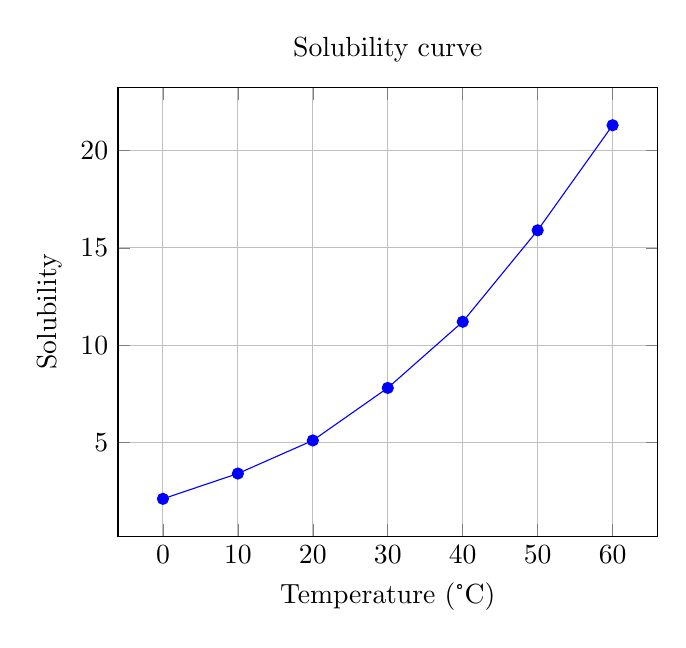
\begin{tikzpicture}
\begin{axis}[
    xlabel={Temperature (°C)},
    ylabel={Solubility},
    title={Solubility curve},
    grid=major
]
\addplot[blue,mark=*] coordinates {
    (0, 2.1) (10, 3.4) (20, 5.1) (30, 7.8)
    (40, 11.2) (50, 15.9) (60, 21.3)
};
\end{axis}
\end{tikzpicture}

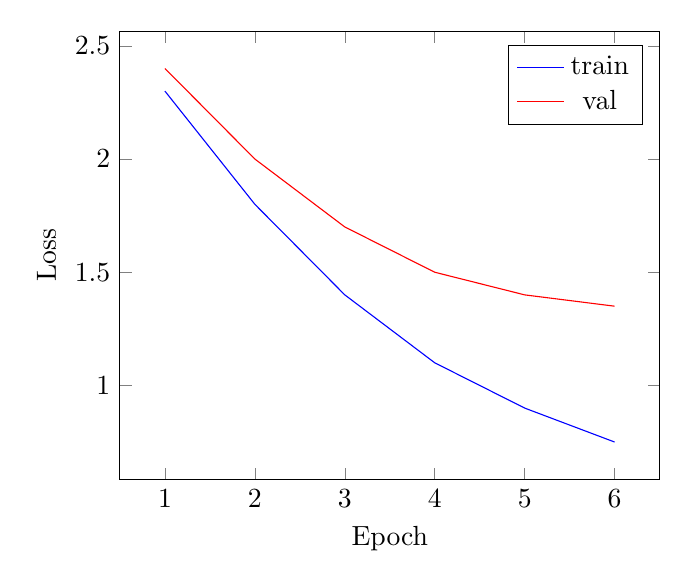
\begin{tikzpicture}
\begin{axis}[
    xlabel={Epoch}, ylabel={Loss},
    legend pos=north east
]
\addplot+[mark=none] coordinates { (1, 2.3) (2, 1.8) (3, 1.4) (4, 1.1) (5, 0.9) (6, 0.75) };
\addlegendentry{train}
\addplot+[mark=none] coordinates { (1, 2.4) (2, 2.0) (3, 1.7) (4, 1.5) (5, 1.4) (6, 1.35) };
\addlegendentry{val}
\end{axis}
\end{tikzpicture}

\end{document}
